\documentclass[tikz,border=5pt]{standalone}
\usepackage[T1]{fontenc}
\usepackage{lmodern}
\usepackage{pgfplots}
\usepgfplotslibrary{groupplots}
\pgfplotsset{compat=1.18}

\definecolor{sapgray}{RGB}{122,122,122}
\definecolor{orblue}{RGB}{76,120,168}
\definecolor{invorange}{RGB}{209,143,0}
% Generated by scripts/create_publication_figures.py from current backtest outputs.
\def\DemandConcentrationCoordinates{(Top 1,12.57) (Top 5,40.34) (Top 10,57.76) (Top 20,73.35)}
\def\SapstaticLabel{SAP-derived}
\def\SapstaticFillCoordinates{(Full cohort,79.99) (Excl. top 5,95.80)}
\def\UniversalrqLabel{SAP-SLT OR}
\def\UniversalrqFillCoordinates{(Full cohort,79.58) (Excl. top 5,95.11)}
\def\LlmpureLabel{LLM-emitted}
\def\LlmpureFillCoordinates{(Full cohort,77.52) (Excl. top 5,91.82)}
\def\FigureTwoFootnote{Generated from the working-days primary backtest; common-feasible cohort n=346.}


\begin{document}
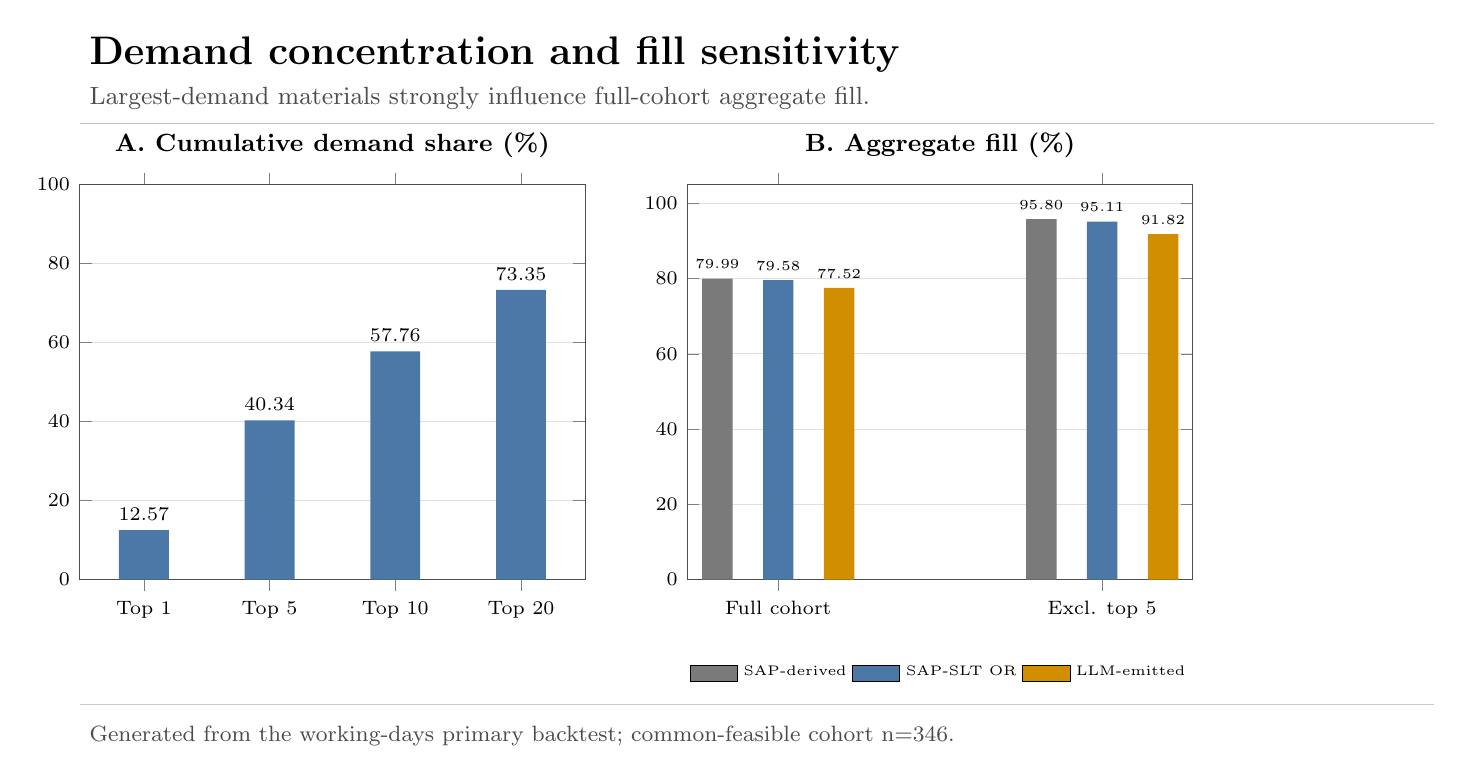
\begin{tikzpicture}
\node[anchor=west,font=\Large\bfseries] at (0,0) {Demand concentration and fill sensitivity};
\node[anchor=west,font=\small,text=black!70] at (0,-0.55)
  {Largest-demand materials strongly influence full-cohort aggregate fill.};
\draw[black!25] (0,-0.88) -- (17.2,-0.88);

\begin{scope}[yshift=-1.65cm]
\begin{groupplot}[
  group style={group size=2 by 1,horizontal sep=1.3cm},
  at={(0,0)},anchor=north west,
  width=8.0cm,height=6.6cm,
  tick label style={font=\scriptsize},
  xticklabel style={font=\scriptsize,align=center},
  title style={font=\small\bfseries},
  axis line style={black!70},
  ymajorgrids=true,grid style={black!12},
  nodes near coords,
  every node near coord/.append style={font=\scriptsize\bfseries},
  enlarge x limits=0.17
]
\nextgroupplot[
  ybar,
  title={A. Cumulative demand share (\%)},
  ymin=0,ymax=100,ytick={0,20,40,60,80,100},
  symbolic x coords={Top 1,Top 5,Top 10,Top 20},
  xtick=data,
  bar width=18pt]
  \addplot[fill=orblue,draw=none] coordinates
    {\DemandConcentrationCoordinates};

\nextgroupplot[
  ybar,
  title={B. Aggregate fill (\%)},
  ymin=0,ymax=105,ytick={0,20,40,60,80,100},
  symbolic x coords={Full cohort,Excl. top 5},
  xtick=data,
  enlarge x limits=0.28,
  bar width=11pt,
  legend style={at={(0.5,-0.19)},anchor=north,legend columns=3,font=\tiny,draw=none},
  nodes near coords={\pgfmathprintnumber[fixed,precision=2,fixed zerofill]{\pgfplotspointmeta}}]
  \addplot[fill=sapgray,draw=none,bar shift=-22pt,area legend,
    every node near coord/.append style={font=\tiny\bfseries,anchor=south}] coordinates
    {\SapstaticFillCoordinates};
  \addlegendentry{\SapstaticLabel}
  \addplot[fill=orblue,draw=none,bar shift=0pt,area legend,
    every node near coord/.append style={font=\tiny\bfseries,anchor=south}] coordinates
    {\UniversalrqFillCoordinates};
  \addlegendentry{\UniversalrqLabel}
  \addplot[fill=invorange,draw=none,bar shift=22pt,area legend,
    every node near coord/.append style={font=\tiny\bfseries,anchor=south}] coordinates
    {\LlmpureFillCoordinates};
  \addlegendentry{\LlmpureLabel}
\end{groupplot}
\end{scope}

\draw[black!20] (0,-8.25) -- (17.2,-8.25);
\node[anchor=west,font=\footnotesize,text=black!70] at (0,-8.65)
  {\FigureTwoFootnote};
\end{tikzpicture}
\end{document}
